
Il \textit{colossal itemset mining} si pone come un'estensione del \textit{frequent itemset mining}
Questa espansione riguarda l'utilizzo di dati
a elevata dimensionalità~\cite{zhu2007mining}, in alcuni domini è possibile infatti che l'insieme degli attributi \(F\) sia di molto superiore al
numero di transazioni nel dataset.

Gli algoritmi tradizionali faticano a processare questi dataset ad alta dimensionalità, così in
letteratura sono state proposte numerose soluzioni.

Carpenter~\cite{DBLP:conf/kdd/PanCTYZ03} è uno dei principali framework per
la ricerca di itemset su dataset ad alta dimensionalità.
Questo algoritmo individua insiemi di feature frequenti generando una versione trasposta del dataset originale, chiamata \textit{TT} un albero, chiamato \textit{row enumeration tree} avente nei nodi tutti i possibili set di transazioni;
successivamente questo viene esplorato utilizzando una ricerca \textit{depth-first}.
In~\cref{fig:chap-3:carpenter} (Fonte:~\cite{pan2003carpenter}) viene presentato un esempio di quanto detto sopra.

\begin{figure}
  \centering
  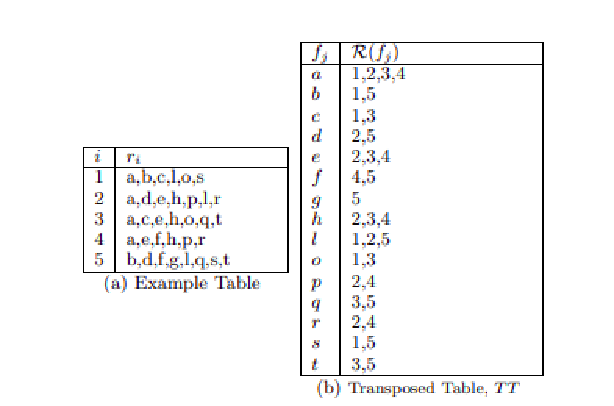
\includegraphics[scale=.7]{/sec-1/CarpenterTableSet.pdf}
  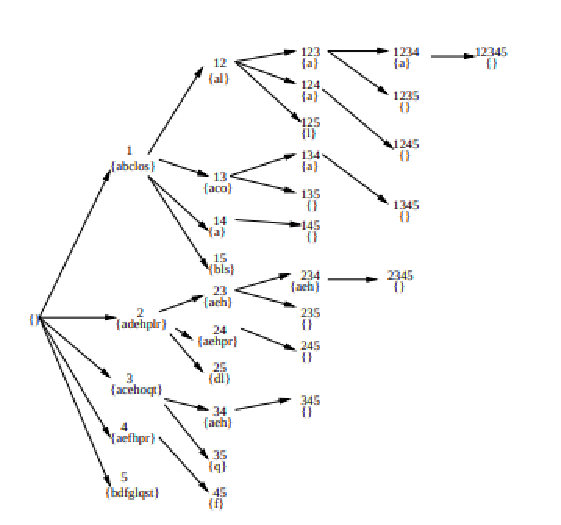
\includegraphics[scale=.7]{/sec-1/CarpenterEnumerationTree.pdf}
  \caption{Esempio di \textit{TT} e \textit{Row Enumeration Tree}}%
  \label{fig:chap-3:carpenter}
\end{figure}

Parlando poi di risultati, Carpenter individua solamente gli itemset chiusi.
Nella sua implementazione, Carpenter è realizzato come algoritmo centralizzato: per evitare infatti
di generare itemset già valutati in iterazione precedenti viene mantenuto un registro globale in
cui sono registrati tutti gli itemset già esplorati.
